\documentclass[a4paper, 12pt]{article}
\usepackage{cite}
\usepackage{multicol, caption}
\usepackage{titling}
\usepackage{graphicx}
\usepackage{tabularx}
\usepackage{subcaption}
\usepackage{url}
\usepackage{amsmath}

\usepackage{listings}
\usepackage{color}

\definecolor{dkgreen}{rgb}{0,0.6,0}
\definecolor{gray}{rgb}{0.5,0.5,0.5}
\definecolor{mauve}{rgb}{0.58,0,0.82}

\lstset{frame=tb,
  language=python,
  aboveskip=3mm,
  belowskip=3mm,
  showstringspaces=false,
  columns=flexible,
  basicstyle={\small\ttfamily},
  numbers=none,
  numberstyle=\tiny\color{gray},
  keywordstyle=\color{blue},
  commentstyle=\color{dkgreen},
  stringstyle=\color{mauve},
  breaklines=true,
  breakatwhitespace=true,
  tabsize=3
}

\newenvironment{Figure}
  {\par\medskip\noindent\minipage{\linewidth}}
  {\endminipage\par\medskip}

%加這個就可以設定字體
\usepackage{fontspec}
%使用xeCJK,其他的還有CJK或是xCJK
\usepackage{xeCJK}
\usepackage[margin=0.6in]{geometry}

%字型的設定可以使用系統內的字型,而不用像以前一樣另外安裝
\setCJKmainfont{DFKai-SB}
\author{}    
\newcommand*{\citenumfont}{}

% Reducing Distance of title and date
\setlength{\droptitle}{-2cm}
\title{\textbf{Fractional Brownian Motion}}
\renewcommand\maketitlehookc{\vspace{-3.5em}}


\begin{document}
    \maketitle     
    \begin{center}
        \begin{tabular}{ccc}
            陳君彥, b04703091 & 劉育嘉, b06902008 & 黃柏豪, b06902124 \\
            b04703091@ntu.edu.tw &
            b06902008@ntu.edu.tw &
            b06902124@ntu.edu.tw
        \end{tabular}
    \end{center}

    \section*{Division of Work}
        陳君彥, b04703091: 
        \begin{itemize}
            \item Data initial processing and calculation tool creation.
            \item Initial creation and testing of XG-boost, LightGBM, and Random Forest Models
        \end{itemize}
        劉育嘉, b06902008:
        \begin{itemize}
            \item Indepth testing of tree based methods
            \item Testing and Creation of select feature models.
        \end{itemize}
        黃柏豪, b06902124:
        \begin{itemize}
            \item Creation and testing of neural network based models.
            \item Creation and testing of blending based models.
        \end{itemize}

        \begin{figure}
            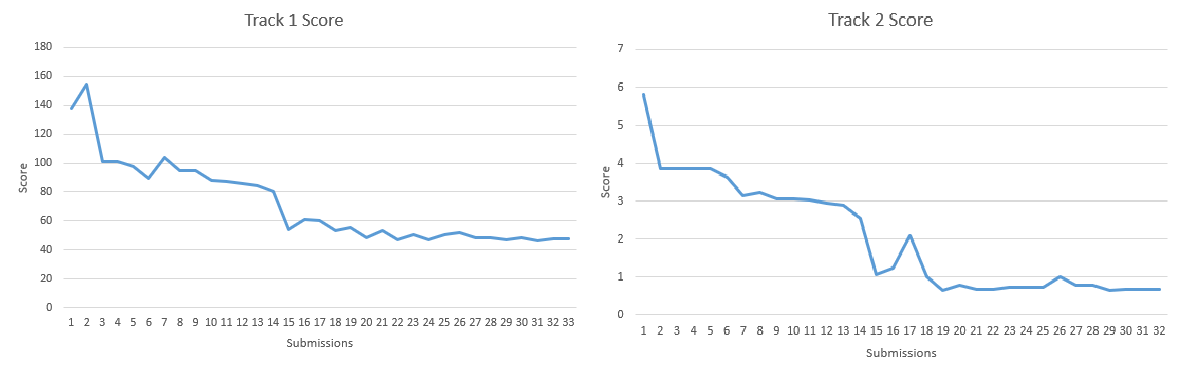
\includegraphics[width=\linewidth]{images/score.png}
            \captionof{figure}{Submission scores of our models.}
            \label{score}
        \end{figure}

        \section{Introduction}
        The goal of this project is to reverse learn model parameters used to simulate a fractional Brownian Motion \cite{fBM} simulation. The parameters used to run this simulation were alpha, mesh size, and penetration rate. We used 2 methods of evaluation, one with "Weighted Mean Absolute Error" (WMAE), and one with "Normalized Absolute Error" (NAE)
        \[WMAE(Y, \hat{Y}) = \frac{1}{n_{samples}}\sum^{n_{samples}}_{i=1}\sum^{3}_{j=1}w_j\mid y_{ij}-\hat{y}_{ij} \mid, NAE(Y, \hat{Y}) = \frac{1}{n_{samples}}\sum^{n_{samples}}_{i=1}\sum^{3}_{j=1} \frac{\mid y_{ij}-\hat{y}_{ij} \mid}{y_{ij}}\]
        
        \newpage

        \begin{multicols}{2}
        \section{Features}
        \subsection{Original Features}
        Our training dataset consists of 47,500 simulations with 10,000 features each. The first 5,000 features represented the mean-square displacements (MSD) of our particles ordered from time = [1,5000]. The second 5,000 features were 50 sets of velocity auto-correlations (VAC) calculated in different methods, ordered by the early VAC being more representative of instataneous velocity, with later VAC being closer to average velocity. Each sets consists of 100 calculation using the respective VAC, with time intervals from t = [1,100].
        
        Our testing sets consists of 2,500 simulations, half of which is tested in the public score, and half hidden in the private score.

            \subsubsection{Feature Importance}
                In the interest of reducing the time need to train our models, we took a look at the feature importance determined by our earlier models and selected those that had importance higher than a given threshold. Through several rounds of testing, we found $10^{-4}$ to perform the best. This allowed us to greatly increase the training iteration count and deepen our original model, giving us increased accuracy with much lower training times.
                
                Something of particular to note is the high reliance of a select few features for each parameter. Due to the lack of professional knowledge in this field and the lack of raw data, we could do little to take advantage of this except to reduce the dimensionality. However we expect that further studies can be improve by generating more features that are centered around these specific features.

            \subsection{Additional Features}
                To gather more physic based features, we also extrapolated some of our own data.

                \begin{Figure}
                    \centering
                    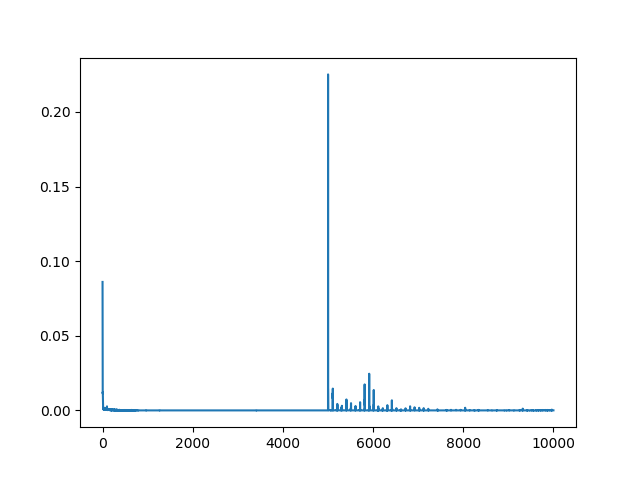
\includegraphics[width=\linewidth]{images/importance_1.png}
                    \captionof{figure}{Feature importance of alpha.}
                    \label{alphafeat}
                \end{Figure}
                \begin{Figure}
                    \centering
                    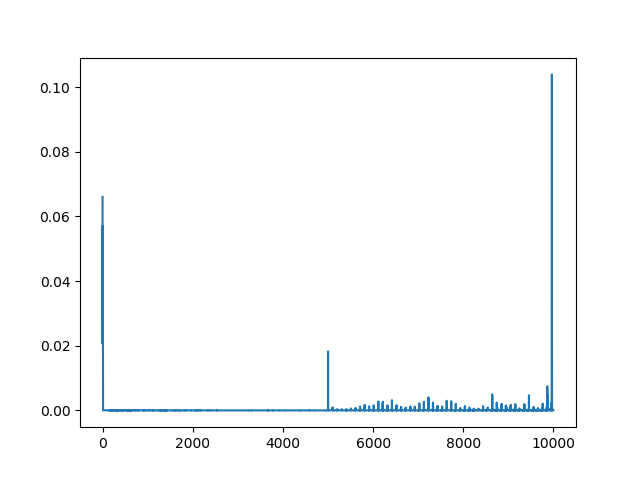
\includegraphics[width=\linewidth]{images/importance_2.png}
                    \captionof{figure}{Feature importance of mesh size.}
                    \label{meshfeat}
                \end{Figure}
                \begin{Figure}
                    \centering
                    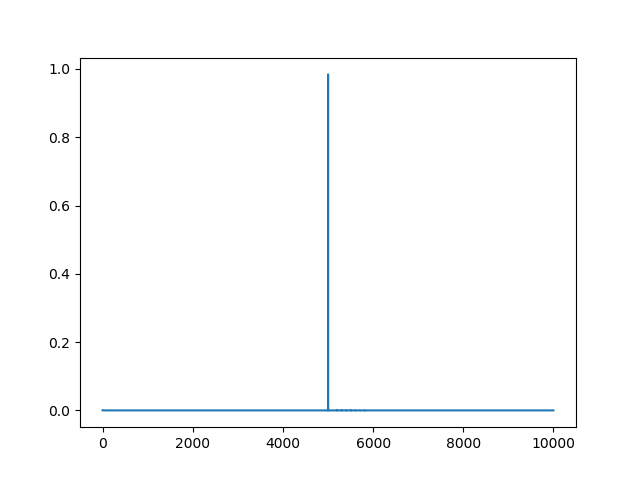
\includegraphics[width=\linewidth]{images/importance_3.png}
                    \captionof{figure}{Feature importance of penetration rate.}
                    \label{penfeat}
                \end{Figure}

                \subsubsection{Average and MinMax}
                    We were interested in having our model be less overfitting and took feature based methods to reduce the feature count. We tried taking the average of every 10 features, which would result in the mean displacement or velocity over a larger time period. We also tried taking the minimum and maximum of each 10 features, which in essence was is a form of data pooling.

                \subsubsection{Square Error on Linear Regression}
                    We assume a particle without external force will go straight forward with constant speed, so the force generated by collision might have something to do with the difference between a linear line and its real value. Therefore, we performed a linear regression compute the variance of those 5000 time intervals, substituting them for the original 5000 features.

                \subsubsection{Alpha feedback}
                    Our models performed exceptionally well on alpha, and so we decided to feedback the results of our third parameter prediction back in as a feature for our other two predictions, giving a slight boost to performance.

        \section{Individual Model Experiments}        
            \subsection{Tree based models}
                \subsubsection{Random Forest}
                We used the models provided in the python package Sci-kit Learn \cite{scikit-learn} for our random forest, with bootstrap enable, estimator count of 50, and a max depth of 9. The following shows the results of our experiments.
                \begin{center}
                    \begin{tabular}{c|ccc}
                        Tree count & Alpha & Mesh Size & Penetration\\
                        \hline
                        50 & 65.72 & 31.92 & 1.96 \\
                        100 & 64.74 & 30.69 & 1.81 \\
                        200 & 64.06 & 29.93 & 1.74 \\
                        300 & 61.02 & 27.20 & 1.54 \\
                        500 & 58.67 & 25.10 & 1.40 \\
                        1250 & 55.07 & 22.40 & 1.23
                    \end{tabular}
                    \captionof{table}{Performance on track 1 for random forest}
                    \label{randForTab}
                \end{center}

                As seen in Table \ref{randForTab}, we achieve moderate performance by simply throwing in the original features into a random forest model. The performance gradually increased with each additional tree count, though the time required to train them starting to get out of hand. Each tree required around 1.5 minute to train when parallelized, meaning training each model for all three features required over 3 hours for each incrementation. Hence we tried it out with a reduced feature set selected using the previously trained model's feature importances.

                
                \begin{center}
                    \begin{tabular}{c|ccc}
                        Tree count & Alpha & Mesh Size & Penetration\\
                        \hline
                        50 & 67.31 & 30.69 & 3.13 \\
                        100 & 67.42 & 30.60 & 3.12 \\
                        200 & 67.35 & 30.65 & 3.11 \\
                        300 & 67.35 & 30.64 & 3.11 \\
                    \end{tabular}
                    \captionof{table}{Performance on track 1 for random forest with reduced input.}
                    \label{randForRedTab}
                \end{center}

                However, as seen in Table \ref{randForRedTab}, the reduced feature set performed poorly, while giving us a very low training time, it failed to beat even the 50 tree count on the regular RF model at 300 trees. We gave up and tried a different approach, reducing the dataset by picking averages of every 10 features.

                
                \begin{center}
                    \begin{tabular}{c|ccc}
                        Tree count & Alpha & Mesh Size & Penetration\\
                        \hline
                        50 & 64.57 & 23.98 & 2.37 \\
                        100 & 64.56 & 23.94 & 2.36 \\
                        200 & 64.56 & 23.86 & 2.36 \\
                        300 & 64.60 & 23.85 & 2.35 \\
                    \end{tabular}
                    \captionof{table}{Performance on track 1 for random forest with averaged features.}
                    \label{randForAvgTab}
                \end{center}

                The results as shown in Table \ref{randForAvgTab} shows that this performed better than the feature selection model, and slighly better than the original model, with a combined score of 90.81 on track 1 and 2.29 on track 2. However, we notice that stop in decrese of the validation error, and recognized that further training would do the model no good.

                \subsubsection{XGBoost}
                    We tried the very popular XGBoost \cite{xgboost} often used in machine learning competitions. XGBoost is a gradient boosting tree model that has an emphasize on reduced tree depth and higher parallelism. This allows us to train a model much faster and allows easier batching on the massive dataset. 

                    
                \begin{center}
                    \begin{tabular}{l|cc}
                        Notes & Track 1 & Track 2\\
                        \hline
                        base & 137.23 & 6.22 \\
                    \begin{tabular}{@{}l@{}}+ filtered data \\ \&alpha feedback \end{tabular} & 48.86 & 0.66 \\
                        + auto tree method & 43.49 & 0.60 \\
                        + tweedie regularizer & 41.70 & 0.38 \\
                        + boot round = 5 & 40.85 & 0.33 \\
                    \end{tabular}
                    \captionof{table}{Performance of xgboost with each additional parameter tuning.}
                    \label{xgboost}
                \end{center}
                    As seen in Table \ref{xgboost}, the xgboost relies heavily on custom tuned parameter, with the base parameters model performing really bad. However, with careful tuning, and the filtered data fed into our model, xgboost provided very respectable data on the validation set. After submitting the results, we found out that the final rounds of tuning had led to the model being overfitted, with the submission score actually being worse than the previous round. We thus stopped our experiments on xgboost here and moved on to a different model.
                \subsubsection{LightGBM}
                    LightGBM \cite{lightgbm} is a very new contender to the scene, with a focus on limiting leaf count rather than xgboost's method of limiting tree depth.

                    In our instant, lightgbm performs much better with base parameters, with learning rate set to 0.01. As seen in Table \ref{lightgbmVal}, it is already in clear competition with xgboost. We also went through the same process of using the predicted alpha to feed back into the model, as well changing to use 'dart' as a boosting method with more iterations. It can be seen from Table \ref{lightgbmSub} that the submission score is also dropping at a steady rate, but then shows signs of overfitting with the last submission, we then started performing regularization to combat the issue.

                    \begin{center}
                        \begin{tabular}{l|cc}
                            Notes & Track 1 & Track 2\\
                            \hline
                            base & 56.80 & 1.52 \\
                            + alpha feedback & 55.87 & 1.20 \\
                            + 1000 iterations + dart & 38.25  & 1.07 \\
                            + 2500 iterations & 30.84 & 0.36 \\
                        \end{tabular}
                        \captionof{table}{Validation performance of lightgbm with each additional parameter tuning.}
                        \label{lightgbmVal}
                    \end{center}

                    \begin{center}
                        \begin{tabular}{l|cc}
                            Notes & Track 1 & Track 2\\
                            \hline
                            base & 60.76 & 2.94 \\
                            + alpha feedback & 59.87 & 2.10 \\
                            + 1000 iterations + dart & 48.23 & 0.92 \\
                            + 2500 iterations & 50.48 & 0.86 \\
                        \end{tabular}
                        \captionof{table}{Submission performance of lightgbm with each additional parameter tuning.}
                        \label{lightgbmSub}
                    \end{center}

                    We tried using the square error on linear regression as a feature, and averaging them out, cutting our feature set down to one tenth of the size, and as seen in Table \ref{lightgbmsquared}, shows that the overfitting issue has been somewhat allieviated.

                    \begin{center}
                        \begin{tabular}{l|cc}
                            Notes & Validation & Submission \\
                            \hline
                            500 iterations & 45.52 & 49.17 \\
                            1000 iterations & 43.27 & 48.13 \\
                        \end{tabular}
                        \captionof{table}{Submission performance of lightgbm with each additional parameter tuning.}
                        \label{lightgbmsquared}
                    \end{center}
            \subsection{Neural network models}
                We used a dense neural network of size 2048-50-1 to predict our three parameters. As the number of features is too big for a neural network, the features were first passed through an autoencoder of size 5000-2048-1024 and train with 'relu' activation on a 5000-2048-1024-2048-5000 model.

            \begin{lstlisting}
def encoder(x, 
    actvation_list = ['relu', 'relu'], 
    layer_list = (2048, 1024),  # dimension for each layer
    name = 'temp', # to specify model file
    use_old = False): # load existing model or not
            \end{lstlisting}

            \subsection{Blending}
        \section{Conclusion}

  \end{multicols}

\vskip 5cm
\bibliography{report}{}
\bibliographystyle{ieeetran}

\end{document}
